\chapter{Evaluación}
\label{cap:evaluacion}

En este capítulo se describe el proceso de evaluación de la aplicación que se ha llevado a cabo. Como ya se puso de manifiesto en el Plan de trabajo (ver Sección \ref{sec:planTrabajo}), la idea inicial era la de realizar una evaluación con usuarios finales y, preferiblemente, en la Facultad de Informática de la UCM, pues ese espacio es nuestro caso de estudio inicial. Debido a la crisis sanitaria y el estado de emergencia declarado en marzo de 2020 a causa de la COVID-19, no ha sido posible la ejecución de dicha evaluación. Sin embargo, conseguimos sobreponernos a este contratiempo y poner de manifiesto la flexibilidad de la aplicación mapeando otro edificio y realizando diversas pruebas sobre este. Este edificio no pudo ser otro que una vivienda. Cabe destacar que este no es el escenario ideal sobre el que se desplegaría una aplicación como Blind Bit, pues el espacio queda considerablemente reducido en comparación con el de una facultad o museo, por ejemplo. A pesar de ello, permite probar el comportamiento de la aplicación en situaciones donde cierta aglomeración de \textit{beacons} es necesaria y poner a prueba el mapeo de un edifico con características distintas al ya planteado en la Sección \ref{sec:mapeo}. En las secciones que siguen se detalla cómo se ha llevado a cabo la adaptación tanto del plan de evaluación como el despliegue de la aplicación en otro edificio.

En la Sección \ref{sec:adaptacionApp} se describen los pasos a seguir, tanto en el servidor (Sección \ref{sub:cambiosServidor_vivienda}) como en el cliente (Sección \ref{sub:cambiosCliente_vivienda}) para poder adaptar la aplicación al nuevo espacio. Por su parte, la Sección \ref{sec:objetivosEval} detalla los objetivos de la evaluación. Las pruebas que se llevaron a cabo a fin de valorar el cumplimiento de estos objetivos se exponen en la Sección \ref{sec:realizYresult} y las conclusiones finales de la evaluación pueden verse en la última sección (Sección \ref{sec:conclusionesEval}).


\section{Adaptación de la aplicación al nuevo edificio}
\label{sec:adaptacionApp}

En esta sección detallaremos los cambios que se han realizado para poder desplegar Blind Bit sobre la vivienda. Veremos tanto los cambios referentes al servidor (Sección \ref{sub:cambiosServidor_vivienda}) como al cliente (Sección \ref{sub:cambiosCliente_vivienda}). Hay que tener en cuenta que ninguno de estos cambios implica la modificación del código de la aplicación, pues esta se ha implementado de manera genérica para permitir su reutilización en nuevos espacios como el que se expone a continuación.

\subsection{Cambios en el servidor}
\label{sub:cambiosServidor_vivienda}

En la Sección \ref{sub:cambiosServidor} se exponen las claves para realizar el mapeo de un nuevo edificio. A continuación veremos cómo se han aplicado estas para el mapeo de la vivienda.


A la hora de enfrentarnos al mapeo de este nuevo edificio hemos seguido la estructura definida en la Sección \ref{sec:mapeo} del Capítulo \ref{cap:descripcionTrabajo} y la hemos representado como archivos XML siguiendo el mismo formato descrito en la Sección \ref{sub:mapeo_xml} del mismo capítulo.

Para ello, lo primero ha sido dividir el edificio en cada una de sus plantas y finalmente dividir estas en cuadrantes únicos. Para realizar esta tarea hay que tener en consideración que tal y como ya habíamos concluido, cada cuadrante ha de contener exactamente un \textit{beacon} que facilite el posicionamiento del usuario en un punto clave o de decisión y que todos aquellos cuadrantes carentes de puntos de decisión y por lo tanto carentes de \textit{beacons} son cuadrantes inservibles que deben juntarse con otros que si contengan un punto de decisión. De esta manera en la Figura \ref{fig:mapeoCasa} podemos ver en rojo la división hecha de cada una de las plantas en sus cuadrantes, cuyos identificadores son los números que aparecen sobre ellos y en los que la ubicación de los \textit{beacons} está representada con un círculo amarillo. Una de las características más importantes que han de tener los cuadrantes en los que dividamos nuestro espacio, además de lo ya mencionado sobre los puntos de decisión y las balizas, es que han de confluir con un cuadrante como máximo por cada punto cardinal (norte, sur, este y oeste) ya que más tarde en el XML se almacenará la información de los cuadrantes con los que cada uno está conectado por el norte, sur, este y oeste, y en cada uno de ellos no puede guardarse más de un identificador.

A diferencia del trabajo realizado en la Facultad de Informática, en este caso sí hemos mapeado las distintas estancias, esto se debe a la naturaleza tan distinta de este edificio que al ser una vivienda particular presenta dimensiones mucho inferiores y por lo tanto, hemos de decidido mapear todo el espacio para añadir complejidad a la guía y que esta no se limite a ir de puerta a puerta.

En la Figura \ref{fig:mapeoCasaPBaja} vemos como hemos dividido la planta baja de la vivienda en 11 cuadrantes, siendo este último el que se corresponde con las escaleras que unen esta planta con el cuadrante 12 de la planta superior. El mapeo de la primera planta se encuentra en la Figura \ref{fig:mapeoCasaPAlta} que como vemos tiene la misma estructura que la planta inferior a excepción de la superficie que se corresponde con los cuadrantes $0$, $1$ y $10$ que desaparecen. Solo hemos incluido dos cuadrantes ya que la división es completamente análoga.

Una vez mapeado el edificio el siguiente paso ha de ser estructurar la información en tres archivos XML que contengan los mismos campos descritos en la Sección \ref{sub:mapeo_xml}. Uno de ellos que haga referencia al esqueleto del edificio y los otros dos que plasmen la información de cada una de las plantas. %En el Apéndice X podemos ver estos archivos XML.



\subsection{Cambios en el cliente}
\label{sub:cambiosCliente_vivienda}

En las Secciones \ref{sub:diseño} y \ref{sub:func_cliente}, revisamos el diseño de la interfaz de la aplicación Blind Bit y su funcionamiento, respectivamente. En cuanto a la interfaz se refiere, es sencillo darse cuenta de que la parte dependiente del edificio corresponde a la pantalla de destinos. Sin embargo, esta está implementada de manera dinámica. Es decir, los nombres de los botones, así como la lista de destinos con la etiqueta correspondiente a los destinos tal y como aparecen en el archivo \textit{destinos.json} del servidor\footnote{Los destinos en la interfaz pueden aparecer con tildes, mayúsculas y otros caracteres especiales que puede no ser posible añadir en el archivo \textit{destinos.json}. Es por ello que se guardan los destinos en dos estructuras, una para la interfaz y otra para la conexión con el servidor.} se guardan en un archivo xml. El archivo donde se guardan estos y otros strings correspondientes a la aplicación, tales como el texto de las instrucciones o la uri del servidor es \textit{listasStringsApp.xml}. Las estructuras referentes a la lista de destinos son \textit{destinos\_array} y \textit{destinosdinamicos\_array}. Mientras que en la primera basta con introducir cada destino en un \textit{<item>}, en la segunda hay que indicar si ese destino tiene un segundo nivel. Por ejemplo, en el caso de la Facultad de Informática tenemos un botón aulas, que no corresponde con un destino sino con el acceso a un segundo nivel donde se muestran las aulas destino disponibles. La estructura que debe seguirse es la siguiente: 


%\lstinputlisting[language=XML]{Imagenes/Evaluacion/destinos_array.xml} 

%\lstinputlisting[language=XML]{Imagenes/Evaluacion/destinosdinamicos_array.xml}

Donde un ``no'' tras la barra indica que no hay un segundo nivel y cualquier otra cadena de strings se entiende como los destinos correspondientes a ese nivel, separados por comas. Este constituye el único cambio necesario para adaptar el cliente a un nuevo espacio.

\section{Objetivos de la evaluación}
\label{sec:objetivosEval}

Debido a la imposibilidad de realizar una evaluación con usuarios. Nos vimos obligadas a reestructurar el \textit{modus operandi} de la evaluación de la aplicación. Concretamente, los objetivos cambiaron, centrándose en el funcionamiento de la misma y dando menos peso a la usabilidad, en la que los usuarios finales tienen un papel decisivo. De esta manera, se decidió establecer cuatro objetivos claros que presentamos a continuación:

\begin{enumerate}
	
	\item \textit{Resolución del problema del posicionamiento:} Una de las funcionalidades principales de la aplicación es, sin duda, la correcta ubicación del usuario. Para ello es necesario que el \textit{beacon} más cercano al usuario sea detectado como el más cercano por la aplicación (ver Sección \ref{sub:func_cliente}). De esta tarea depende no solo el inicio de la ruta sino el seguimiento de toda ella, pues en todo momento debemos conocer el cuadrante donde se encuentra el usuario para que la aplicación pueda responder en consecuencia. Una mala ubicación del usuario podría provocar que el usuario se pierda debido a indicaciones que no corresponden con su posición o, en casos más graves, el tropiezo o golpeo del usuario con un obstáculo del que no ha sido advertido.
	
	Cabe destacar que en el posicionamiento influye no solo la correcta implementación del código, sino también la ubicación de los \textit{beacons}, que debe adaptarse a las necesidades específicas de cada edificio. 
	
	\item \textit{Generación de instrucciones correctas:} Teniendo en cuenta la ubicación del usuario y el camino que ha seguido, es primordial que la aplicación sea capaz de generar instrucciones correctas. Tanto los giros como la señalización de puntos de interés como los ascensores o el destino debe corresponderse con la ubicación real de estos, tal y como se establece en los archivos xml (ver Sección \ref{sub:mapeo_xml}).
	
	\item \textit{Precisión de las instrucciones:} Además de que las instrucciones sean correctas, hay que evaluar que el usuario las recibe en el momento adecuado. Esto está claramente relacionado con el posicionamiento, pues el momento de indicación de la ruta se basa en cuándo el usuario llega a un determinado cuadrante. Sin embargo, se debe prestar especial atención a las posibles variaciones que pueden darse (una instrucción puede darse con cierta antelación o, por el contrario, una vez pasado el punto óptimo) y evaluar si esa flexibilidad es asumible para el usuario.
	
	\item \textit{Ejecución correcta en caso de usuario perdido:} Este es un punto importante, pues no debemos asumir que el usuario va a seguir siempre la ruta, puede ocurrir que por diversos motivos (una distracción, un obstáculo o el propio fallo de la aplicación) el usuario se desvíe de la ruta. En ese caso no solo se debe identificar el problema sino también saber reconducir al usuario al destino deseado. 
		
\end{enumerate}


\section{Realización y resultados de la evaluación}
\label{sec:realizYresult}

La realización de la evaluación no pudo darse en el edificio objetivo de nuestro estudio (la Facultad de Informática de la UCM) debido a la imposibilidad de acceder a él. Sin embargo, conseguimos sobreponernos a este contratiempo y poner de manifiesto la flexibilidad de la aplicación mapeando otro edificio y realizando diversas pruebas sobre este. Este edificio no pudo ser otro que una vivienda. Cabe destacar que este no es el escenario ideal sobre el que se desplegaría una aplicación como Blind Bit, pues el espacio queda considerablemente reducido en comparación con el de una facultad o museo, por ejemplo. A pesar de ello, permite probar el comportamiento de la aplicación en situaciones donde cierta aglomeración de \textit{beacons} es necesaria y poner a prueba el mapeo de un edifico con características distintas al ya planteado en la Sección \ref{sec:mapeo}.

\subsection{Mapeo del nuevo espacio}

Como ya se avanzaba en la introducción, el edificio sobre el que se basa la evaluación es una vivienda. En la Figura \ref{fig:mapeoCasa} vemos el resultado del mapeo, donde el número de cuadrante está recuadrado en negro, la posición de los beacons en amarillo y los cuadrantes vienen delimitados por las líneas rojas y las paredes de la vivienda. Como muestra la Figura \ref{fig:mapeoCasaPAlta}, el mapeo de la planta alta se ha reducido a dos cuadrantes, pues son suficientes para \textit{testear} las rutas que incluyen un cambio de planta ya que la estructura es análoga a la de la planta baja.


\begin{figure}[t!]
	\centering
	
	\subfloat[Mapeo de la planta baja de la vivienda]{
		\label{fig:mapeoCasaPBaja}
		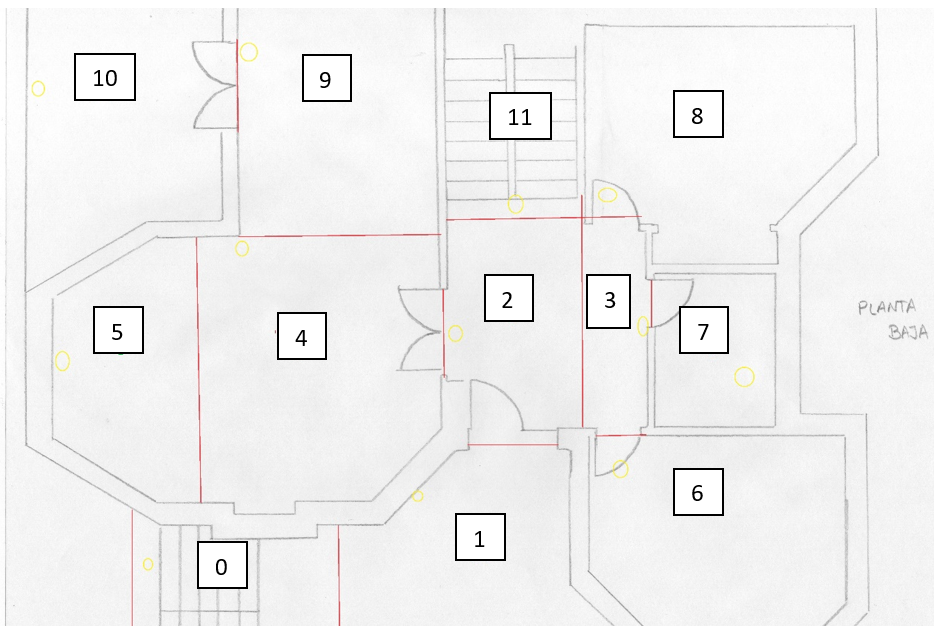
\includegraphics[width=0.8\textwidth]{Imagenes/Evaluacion/planoCasaPBaja}}
	
	\subfloat[Mapeo de la planta alta de la vivienda]{
		\label{fig:mapeoCasaPAlta}
		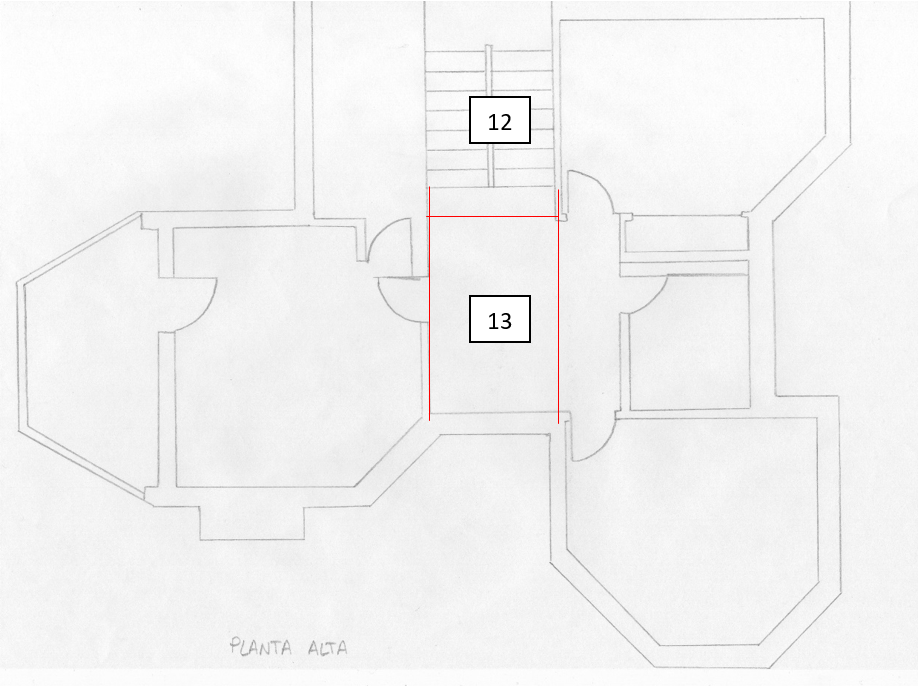
\includegraphics[width=0.8\textwidth]{Imagenes/Evaluacion/planoCasaPAlta}}\\
	
	\caption{Mapeo de la vivienda}
	\label{fig:mapeoCasa}
\end{figure}

A continuación se describen las pruebas realizadas y se analizan los resultados obtenidos.

\subsection{Seguimiento de la ruta}
En esta sección se detallan las pruebas realizadas asumiendo que el usuario no va a salir de la ruta. Sin embargo, algunas de ellas están diseñadas para reproducir situaciones extremas como la pérdida de un \textit{beacon} o rutas potencialmente complicadas.


\subsubsection{Ruta del cuadrante $0$ al cuadrante $10$}
\label{subsub:0al10}
La primera ruta de la evaluación consiste en realizar la ruta desde el cuadrante $0$ hasta el cuadrante $10$ sin salir de la ruta. En esta se debe prestar especialmente atención a las instrucciones de giro, pues son constantes durante toda la ruta. Además, no debemos olvidar que la aplicación emite distintas vibraciones en función de la dirección de giro. Estas vibraciones deben quedar lo suficientemente claras para el usuario. 

Este recorrido se realizó varias veces a fin de encontrar irregularidades en la ruta. A continuación se detallan las conclusiones obtenidas:

\begin{itemize}
	\item Las instrucciones generadas por la aplicación son correctas y, en la mayor parte de los casos, se indican al usuario en el momento adecuado.
	
	\item Las vibraciones asociadas a los giros y a la llegada del destino son lo suficientemente distintas para que el usuario pueda distinguirlas.
	
	\item En dos ocasiones las instrucciones correspondientes a los cuadrantes $1$ y $2$ se dieron demasiado pronto. Esto puede deberse a que el \textit{beacon} del cuadrante $1$ está situado en el exterior y que, una vez que se avanza hacia la puerta que separa los cuadrantes $1$ y $2$, la distancia que hay entre ellos es reducida.
	
	\item En una de las ocasiones el \textit{beacon} asociado al cuadrante $4$ no fue detectado por la aplicación, provocando la pérdida de esa instrucción (en las pruebas siguientes se detalla el comportamiento de la aplicación en este caso. Ver Secciones \ref{subsub:0al10sin4} y \ref{sub:usuarioPerdido}).
	
	\item Una vez se ha llegado al destino, la posición del mismo se indica correctamente en función de la dirección desde la que proviene del usuario.
	
\end{itemize}

\subsubsection{Ruta del cuadrante $1$ al cuadrante $10$}

Este caso es prácticamente idéntico al anterior (Sección \ref{subsub:0al10}), con la única diferencia que se pone a prueba el posicionamiento inicial del usuario. Tras comprobar que las instrucciones en el cuadrante $1$ se daban antes de lo previsto en algunas ocasiones, se decidió empezar la ruta en este cuadrante. De esta manera la aplicación debía detectar el \textit{beacon$1$} como \textit{beacon} más cercano. Se hicieron cinco pruebas y se pudo comprobar que en dos ocasiones este posicionamiento no se realizó de manera correcta. En uno de ellas el \textit{beacon} más cercano detectado por la aplicación fue el $4$ (lo que puede ser provocado porque la separación entre el $4$ y el $1$ es una ventana) y en otra el $2$ (cuya posible explicación  ya fue mencionada en la Sección \ref{subsub:0al10}).

\subsubsection{Ruta del cuadrante $0$ al cuadrante $10$, eliminando el \textit{beacon} del cuadrante $4$}
\label{subsub:0al10sin4}

En este caso se ha vuelto a repetir la ruta del cuadrante $0$ al $10$ con la particularidad de que el \textit{beacon$4$}\footnote{Asumiremos que \textit{beaconX} es el \textit{beacon} asociado al cuadrante X.} fue eliminado de la ruta. Sin embargo, no provocamos la situación de que el usuario se saliera de la ruta (como sería lógico en esta situación, pues la instrucción de giro del cuadrante $4$ se pierde), continuamos por el cuadrante $9$. De esta manera la aplicación no notifica que el usuario se ha perdido, pues sigue en la ruta. A pesar de que la instrucción indicada en el cuadrante $9$ fue la correcta (giro a la izquierda), la aplicación tardó demasiado. Esto se debe a que el umbral de la variable \textit{numPasosPerdidos}, que identifica el momento en el que el usuario puede haberse perdido (ver Sección \ref{sub:func_cliente}), es demasiado elevado para este edificio, donde las distancias entre \textit{beacons} son pequeñas.


\subsubsection{Ruta del cuadrante $1$ al cuadrante $5$, eliminando el \textit{beacon} del cuadrante $2$}
\label{subsub:1al5sin2}

Este caso es interesante, pues, a pesar de que se ha eliminado uno de los \textit{beacons} correspondientes a una intersección, la información de giro del cuadrante $2$ no se pierde. Esto se debe a que, como la aplicación es capaz de avisar de los cambios de dirección con antelación, en el cuadrante $1$ ya se indica al usuario que, tras avanzar unos metros, debe girar a la izquierda. Bien es cierto que se pierde precisión, pues el usuario no percibe la instrucción de giro en el momento en el que debe realizarse, ni la confirmación sonora y vibración asociada a esta. Sin embargo, el hecho de que se den instrucciones por adelantado favorece que el usuario permanezca en la ruta aún cuando alguna instrucción se pierda. 

Particularmente para esta ruta, el giro del cuadrante $2$ es el único que hay que realizar y, debido a esto, es más fácil que el usuario no se pierda. Si, por el contrario, el destino hubiera sido el cuadrante $10$, es probable que el usuario no hubiera llegado a recibir la instrucción de giro a la derecha del cuadrante $4$ tampoco. Esto se debe a que la aplicación necesita un tiempo (llegar a un número de pasos perdidos) para decidir si el usuario se ha perdido. De esta manera, cuando el usuario llega al cuadrante $4$ la aplicación sigue a la espera del cuadrante $2$ (el umbral de \textit{numPasosPerdidos} es demasiado alto. Ver funcionamiento en la Figura \ref{fig:diag_clienteSeguimientoRuta}). Esto implica que el usuario se salga de la ruta. Caso que abordamos en la Sección \ref{sub:usuarioPerdido}.


\subsubsection{Ruta del cuadrante $1$ al cuadrante $13$}

En este caso, lo que se quería evaluar eran las instrucciones referentes al cambio de planta. Como ya se comentó en la Sección \ref{sub:cambiosServidor}, el código asume que los cambios de planta se realizan por medio de ascensores. Esta información se ha ignorado en esta ocasión, pues solo se disponía de escaleras. 

De la ruta desde el cuadrante $1$ al $13$ destacamos un punto importante, que es la anticipación de los ascensores en el cuadrante $2$ gracias a la información adicional generada. Esto avisa al usuario del cambio de planta. Una vez en el cuadrante $11$, la aplicación indica al usuario a qué planta se debe dirigir y en qué dirección se encuentran los ascensores (en este caso, delante del usuario). Una vez en la planta superior, la instrucción del cuadrante 12 continua teniendo en cuenta la nueva orientación del usuario (continúa recto). 

\subsubsection{Ruta del cuadrante $13$ al cuadrante $8$}
\label{subsub:13al8}

La finalidad de esta ruta es, principalmente, comprobar el comportamiento de la aplicación en el \textit{hall} de la planta baja, así como el cambio de planta inverso. 

El problema que surge aquí es que los giros que hay que realizar en la planta baja son bastante tediosos. Por un lado, la ubicación del \textit{beacon$2$} favorece que la instrucción de giro hacia el \textit{beacon$3$} tarde demasiado en llegar. Una vez que se proporciona esta instrucción, el cuadrante $3$ vuelve a hacer girar al usuario hacia el $8$, lo que provoca cierta confusión. De igual manera se probó la ruta inversa, desde el cuadrante $8$ al $13$, y el resultado fue análogo.


\subsubsection{Ruta del cuadrante $9$ al cuadrante $13$}
\label{subsub:9al13}

Como la ruta por el \textit{hall} de la planta baja había resultado tediosa en el caso anterior, se hizo una prueba desde el otro extremo. Esta vez la ubicación del \textit{beacon$2$} favorece el giro del usuario para encontrar el ascensor (escaleras en este caso). De esta manera la ruta resulta mucho más natural y organizada que en el caso anterior.

\subsection{Usuario perdido}
\label{sub:usuarioPerdido}

En esta sección se expone el comportamiento de la aplicación cuando el usuario sale de la ruta, basado en ejemplos de ejecución reales. 

En la Sección \ref{subsub:0al10sin4} vimos un caso en el cual era probable que un usuario se desviara de la ruta, debido a la pérdida de la instrucción de giro asociada al cuadrante $4$. De esta manera el usuario continuaría hasta llegar al cuadrante $5$. Es entonces cuando la aplicación detecta que el usuario se ha salido de la ruta e indica al usuario que debe volver por la dirección en la que venía y le permite iniciar de nuevo la ruta al destino desde su posición actual. Como ya se ha comentado, esta indicación se da con cierto retraso debido a que el valor que debe alcanzar la variable \textit{numPasosPerdidos} es demasiado elevada para este edificio. 

Además, la aplicación está preparada para el caso en el que no se detecte ningún \textit{beacon}. Si no se produjera ninguna detección transcurrido un tiempo (determinado por una variable umbral), la aplicación advierte al usuario de la situación indicándole que debe posicionarse dentro del edificio\footnote{Se asume que si ningún \textit{beacon} es detectado es porque el usuario no se encuentra dentro del edificio o la zona mapeada}. Esta situación se reprodujo avanzando hacia la izquierda del cuadrante $0$ y eliminando los \textit{beacons} más próximos a esa zona para provocar que ninguno de ellos fuera detectado.

A pesar de que no ha sido detallado expresamente durante la realización de las pruebas, hay que mencionar que el resto de funcionalidades como el modo silencio, la repetición de la última instrucción, el modo instrucciones detalladas y la finalización anticipada de la ruta también fueron comprobados, sin destacar ningún comportamiento extraño o inesperado.

\section{Conclusiones de la evaluación}
\label{sec:conclusionesEval}

En las pruebas realizadas y descritas en la Sección \ref{sec:realizYresult} se ha puesto de manifiesto el comportamiento de la aplicación en situaciones normales y extremas. Abordando también aquellos casos en los que el usuario se pierde. En esta sección se exponen los puntos más relevantes obtenidos tras el análisis de las situaciones vistas.


\begin{itemize}
	\item \textit{El código de la aplicación funciona de la manera esperada:} A lo largo de las numerosas rutas de prueba se ha podido comprobar que las instrucciones, vibraciones y sonidos se reproducen e indican al usuario de la manera esperada. No se ha apreciado ningún comportamiento inesperado o erróneo. 
	
	\item \textit{El mapeo del edificio juega un papel primordial:} Como se puede observar en las Secciones \ref{subsub:13al8} y \ref{subsub:9al13} la disposición de los cuadrantes y \textit{beacons} puede facilitar la ruta al usuario en gran medida. Por ello, cuantos menos cuadrantes más sencilla será la ruta. La ubicación de los \textit{beacons} debe ser lo más neutra posible. Es decir, que no favorezca más una ruta que otra.
	
	\item  \textit{Se debe ajustar el umbral de la variable numPasosPerdidos al espacio comprendido entre los beacons:} Han sido varias las ocasiones donde se ha puesto en evidencia que las indicaciones sobre el cambio de ruta debían haberse proporcionado con anterioridad. Para solucionarlo basta con reducir este umbral, teniendo en cuenta que el tiempo que tarda en recorrer un espacio una persona con discapacidad visual suele ser ligeramente mayor.
	
	\item \textit{La generalidad de la aplicación:} Debido a las circunstancias, la evaluación de la aplicación ha sido realizada en un edificio distinto a la Facultad de Informática de la UCM. Gracias a una implementación general, apenas dependiente del espacio donde se despliega, el esfuerzo para poder adaptarla queda reducido a la realización de los archivos xml y json de la Sección \ref{sec:mapeo}.
	
	\item \textit{Ventajas de las instrucciones e información adicional anticipadas:} Como pudimos ver en la Sección \ref{subsub:1al5sin2}, el hecho de que las instrucciones de giro se avisen con un cuadrante de antelación prepara al usuario para el cambio de dirección, favoreciendo que este no se salga de la ruta, y, en caso de que el \textit{beacon} de la intersección no se detecte, facilita que la información de la ruta persista. Lo mismo ocurre con la información adicional, sobre todo en el caso de los ascensores, pues permite al usuario identificar que debe cambiar de planta para llegar a su destino por adelantado.

\end{itemize}


